\documentclass[a4paper,12pt]{article}

\usepackage[utf8]{inputenc}
\usepackage{amsmath, amssymb}
\usepackage{graphicx}
\usepackage{float}
\usepackage{caption}
\usepackage{geometry}
\usepackage{hyperref}
\usepackage{enumitem}
\usepackage[ngerman]{babel}
\usepackage{mathptmx}

\geometry{a4paper, margin=1in}

\title{Laborbericht: Analog/Digital- und Digital/Analog-Wandler}
\author{Helen Klos \\Matrikelnummer: 2222449 \\ \\Sandro Fahrion \\Matrikelnummer: 6684592}
\date{26.-27.09.2024}

\begin{document}
\hyphenpenalty=1000
\exhyphenpenalty=1000
\sloppy
\setlength{\emergencystretch}{5pt}

\maketitle

\begin{figure}[H]
    \centering
    
\includegraphics[width=1.0\textwidth]{../Quellen/Labor1/Titelbild.jpg}
\end{figure}
\newpage
\tableofcontents
\newpage

\section{Einführung und Überblick}
In verschiedenen technischen Bereichen und modernen Systemen spielen Datenerfassungen eine zentrale Rolle. Die Kommunikation zwischen Menschen und einem System muss für beide Seiten verständlich gestaltet werden. Menschen können analoge Werte verstehen, welche in dieser Form von Systemen, wie beispielsweise Computern nicht verstanden werden können, da diese nur mit binären Daten arbeiten können. Hier werden Analog-Digital-Converter (ADCs) und Digital-Analog-Converter (DACs) entscheidend. Sie kommen sowohl in industriellen Anwendungen als auch im Alltag zum Einsatz.\\\\
Analog-Digital-Converter wandeln analoge Signale in digitale Signale um, dass das System diese verarbeiten kann. Ein klassisches Beispiel für den Einsatz eines ADCs ist bei der Umwandlung von beispielsweise Temperatuen in digitale Signale. Der ADC tastet das analoge Signal also in festgelegten Intervallen ab und ordnet jedem Abtastwert einen digitalen Code zu.\\
DACs funktionieren genau umgekehrt. Sie wandeln digitale Signale zurück in die analoge Form. Ein Beispiel hierfür wäre das Umwandeln von Audiosignalen in einen, von Menschen hörbaren, Ton, der über Lautsprecher oder Kopfhörer abgespielt werden kann.\\\\
In diesem Laborbericht werden, mit einem ADC und einem DAC durchgeführte, Versuche beschrieben. Diese dienten zum Untersuchen wichtiger Parameter und Funktionen dieser Bauteile. Wichtige Parameter sind beispielsweise die Integrale Nichtliearität, die Differentiell Nichtlinearität und die Konversionszeit. Diese beschreiben die Qualität und die Genauigkeit der verwendeten Bauteile. Weitere untersuchte Eigenschaften sind die Monotonie und das Einschwingverhalten. Der Bericht unterteilt sich in Versuch 1 (ADC) und Versuch 2 (DAC). Es werden jeweils der Aufbau der Schaltung, die verwendeten Bauteile und Geräte, sowie die Versuchsdurchführung mit Messergebnis-Auswertung berichtet.
\newpage

\section{Versuch 1: Analog/Digital-Converter (ADC)}

\subsection{Zielsetzung}
Im Rahmen des ersten Labor-Experiments wurde das Ziel verfolgt, durch verschiedene Messungen die Eigenschaften und Funktionsweise eines ADCs zu untersuchen. Hierzu sollte zuerst eine Schaltung mit einem ADC aufgebaut und in Betrieb genommen werden. Anhand dieser Schaltung sollte im Anschluss die Integrale Nichtlinearität über den Gesamtbereich, die Differentielle Nichtlinearität im mittleren Bereich sowie die Konversionsrate durch entsprechende Messungen ermittelt werden.\\\\Diese Parameter beschreiben die Qualität und Genauigkeit des ADCs. Die integrale Nichtlinearität ist die maximale Abweichung zwischen dem gemessenen und dem idealen Verlauf, weshalb diese idealerweise null sein. Die integrale Nichtlinearität wird im Gegensatz zur differentiellen Nichtlinearität über den Gesamtbereich gemessen. Die differentielle Nichtlinearität vergleicht die Abweichung jeder Funktionsstufe einzeln. Diese sollte ebenfalls im Optimalfall null sein, darf jedoch $\pm1$ nicht überschreiten. Die Konversionsrate beschreibt die Häufigkeit der Umwandlungen der analogen in digitale Werte in Abhängigkeit der Zeit.\\\\
Die gemessenen Daten sind sowohl in einer Tabelle darzustellen, als auch teilweise grafisch aufzubereiten.

\subsection{Messgeräte und Bauteile}
Verwendete Geräte und Zubehör:
\begin{itemize}
\item Netzgerät (NEP-8323)
\item Fluke 87 V True RMS Multimeter
\item Keysight Oszilloskop (DSOX1102A)
\item Bananenkabel (mehrere: rot, blau, schwarz)
\item Sicherheits-Klemmprüfspitze (2 Stück)
\item Oszilloskop BNC Tastkopf mit Masseklemme
\item Steckkabel (mehrere: im Idealfall verschiedene Farben)
\item Steckbrett\\
\end{itemize}

\noindent Verwendete Bauteile:
\begin{itemize}
\item A/D Converter (ADC080x)
\item 10 Segment LED-Bar (OSX10201-B)
\newpage
\item Kondensatoren: 
	\begin{itemize}
	\item 10 µF "Tantalum"
	\item 0,1 µF (2 Stück)
	\item 150 pF
	\end{itemize}
\item Widerstände: 
	\begin{itemize}
	\item 1k$\Omega$
	\item 10k$\Omega$
	\item 8 x 1 k$\Omega$ Widerstandsnetzwerk
	\end{itemize}
\end{itemize}

\subsection{Aufbau der Schaltung}
Zu Beginn des Versuchs wurden alle benötigten Geräte, Bauteile und Zubehör wie Kabel etc. an den Platz geholt und zurecht gelegt. Anschließend wurde die Schaltung mit dem ADC aufgebaut (siehe Figure 2). Mithilfe der Schaltbild-Skizze, aus einem Datenblatt (siehe Figure 1), konnte die LED-Bar, sowie die Kondensatoren und Widerstände, mit den Steckkabeln, an den richtigen Pins angeschlossen werden. Hierzu wurden unterschiedliche Farben und möglichst kurze Kabel verwendet, um die Übersichtlichkeit zu steigern. Die Platzierung des, in der Schaltbild-Skizze zwischen ADC und LED-Bar liegende, Widerstandsnetzwerks wurde mit der LED-Bar vertauscht, da die einzelnen Widerstände des Netzwerks an einem Ende alle miteinander verbunden waren.\\\\Zusätzlich galt es zu beachten, dass manche Bauteile auf die Digital-, und andere hingegen auf die Analog-Masse geschaltet werden mussten. Pin 8 und Pin 9, somit die Eingangsspannung und die Referenzspannung, werden auf die Analog-Masse geschalten, die restlichen, auf Masse geschalteten, Pins werden mit der Digital-Masse verbunden. Hier gilt es zu beachten, dass der Pin, an den die Eingangspannung angelegt wird, mit einem 1k$\Omega$ Schutzwiderstand, gegen Überspannung und mit einem 100 µF Kondensator, gegen Einstreuungen, gesichert werden soll.
Des Weiteren musste, für die Messungen der Konversionsrate, die Clockfrequenz des ADC (ca. 600 kHz) berücksichtigt werden.

\begin{figure}[H]
    \centering
    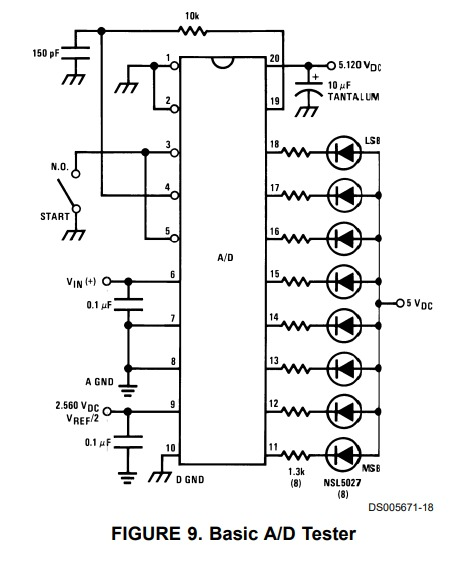
\includegraphics[width=0.5\textwidth]{../Quellen/Labor1/Versuch1/Schaltung ADC mit LEDBar.png}
\caption{Schaltbild-Skizze aus Datenblatt https://www.farnell.com/datasheets/10421.pdf}
\end{figure}

\noindent Bereits während der Vorbereitung wurden die Versorgungsspannung und die Referenzspannung auf jeweils 5,12 V und die Strombegrenzung auf 200 mA  eingestellt, um keine Bauteile durch Überlastung durch zu viel Spannung oder Strom zu beschädigen. Diese Netzgeräte wurden jedoch anschließend wieder ausgeschalten, um nicht Gefahr zu laufen Geräte oder Bauteile kaputt zu machen, während die Schaltung noch nicht von einer Betreuung abgenommen wurde. Ein Weiterer Schritt der Vorbereitung, war das Anschließen des Fluke Multimeters an das Steckbrett, durch Bananenkabel.

\begin{figure}[H]
    \centering
    \includegraphics[width=0.8\textwidth]{../Quellen/Labor1/Versuch1/Schaltungsaufbau-Versuch1.jpeg}
    \caption{Schaltungsaufbau}
\end{figure}

\noindent Nach dem Aufbau der Schaltung, erfolgte zunächst eine Selbstprüfung und anschließend eine Abnahme und Freigabe für die anstehenden Messungen, von einer Betreuung. Im Anschluss wurde die Schaltung in Betrieb genommen, indem zuerst die zuvor eingestellte Versorgungsspannung, gefolgt von der Referenzspannung, sowie der Signalspannung, angelegt wurde. Anschließend wurde die Funktion getestet und die Messungen konnten durchgeführt werden.

\subsection{Messungs-Durchführungen}
\subsubsection*{Messung der Integralen Nichtlinearität (INL)}
Bevor mit den Messungen begonnen wurde, wurde der Eingangsspannungs-Bereich zur anschließend folgenden Protokollierung in 16 gleich große Bereiche unterteilt und notiert. Diese Bereiche sind als Bitmuster in Table 1 nachvollziehbar. Des Weiteren wurde durch diese, die gegebene Referenzspannung U\textsubscript{ref}=5.12 V und U\textsubscript{LSB}=20 mV die zu erwartende Spannung berechnet.\\
Nun wurde die Signalspannung von null bzw. von 0,31 V startend soweit erhöht, bis das Bitmuster gerade auf das gewünschte Muster umspringt. Das Umspringen der Bitmuster kann an der LED-Bar abgelesen werden. Eine leuchtende LED stellt eine null dar. Leuchtet eine LED nicht, bedeutet das eine eins. Gelesen wird von unten nach oben. Die untersten zwei LEDs leuchten in diesem Versuchsaufbau nie, da nur 8 Segmente der 10 Segment LED-Bar verwendet wurden.\\
Für jedes Bitmuster wurde dann die notwendige Eingangsspannung mit dem Fluke Multimeter gemessen und notiert, sowie die Differenz zur erwarteten Spannung, bzw. zur Idealgeraden berechnet. Die Daten sind in Table 1 aufgeführt. Die Verteilung dieser Spannungs-Abweichungen zur Idealgeraden wurden anschließend als Histogramm dargestellt (siehe Figure 3).\\



\setlength{\tabcolsep}{14pt}

\begin{table}[H]
    \centering
    \begin{tabular}{|c|c|c|c|c|}
        \hline
        x = & Bitmuster & U\textsubscript{erwartet} & U\textsubscript{gemessen} & $\Delta$U \\
        \hline
        0 & 00000000 & -0.01 V & - & - \\
        16 & 00010000 & 0.31 V & 0.318 V & 0.008 V \\
        32 & 00100000 & 0.63 V & 0.633 V & 0.003 V \\
        48 & 00110000 & 0.95 V & 0.956 V & 0.006 V \\
        64 & 01000000 & 1.27 V & 1.278 V & 0.008 V \\
        80 & 01010000 & 1.59 V & 1.605 V & 0.015 V \\
        96 & 01100000 & 1.91 V & 1.923 V & 0.013 V \\
        112 & 01110000 & 2.23 V & 2.246 V & 0.016 V \\
        128 & 10000000 & 2.55 V & 2.563 V & 0.013 V \\
        144 & 10010000 & 2.87 V & 2.882 V & 0.012 V \\
        160 & 10100000 & 3.19 V & 3.196 V & 0.006 V \\
        176 & 10110000 & 3.51 V & 3.526 V & 0.016 V \\
        192 & 11000000 & 3.83 V & 3.841 V & 0.011 V \\
        208 & 11010000 & 4.15 V & 4.158 V & 0.008 V \\
        224 & 11100000 & 4.47 V & 4.474 V & 0.004 V \\
        240 & 11110000 & 4.79 V & 4.79 V & 0.000 V \\
        255 & 11111111 & 5.09 V & 5.091 V & 0.001 V \\
        \hline
    \end{tabular}
    \caption{Messergebnisse Integrale Nichtlinearität}
\end{table}


\begin{figure}[H]
    \centering
    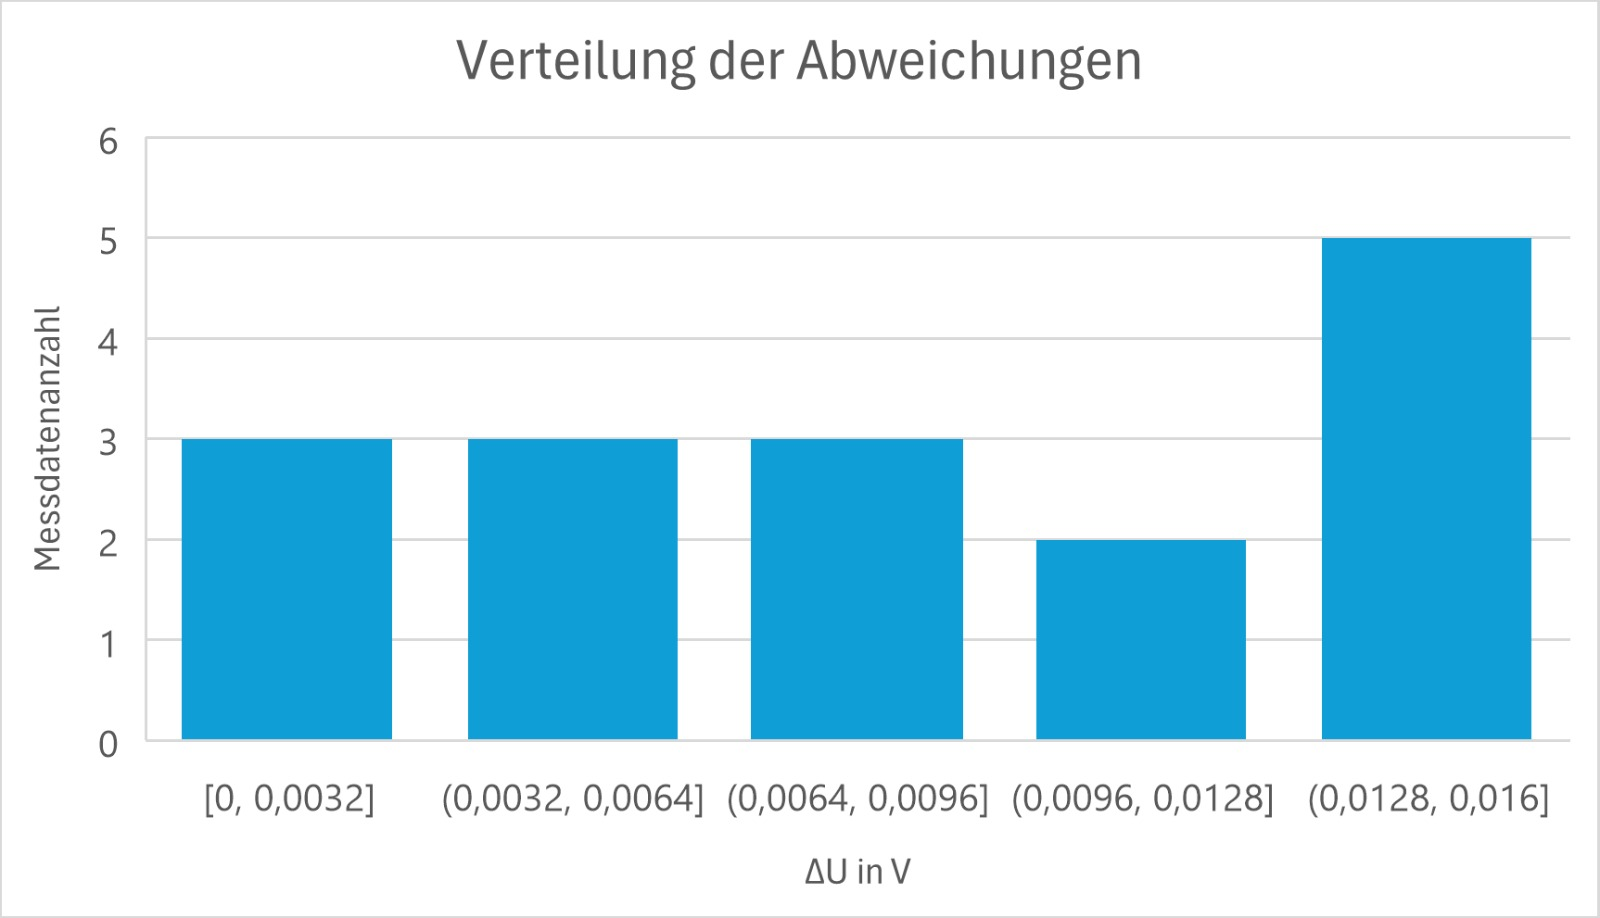
\includegraphics[width=0.9\textwidth]{../Quellen/Labor1/Versuch1/HistogrammAbweichungs-Verteilung.png}
    \caption{Histogramm Verteilung der Abweichungen zur Idealgeraden}
\end{figure}

\noindent Beim Vergleich der gemessenen Spannung mit der erwarteten Spannung, lässt sich feststellen, dass die Werte sich zwar unterscheiden, jedoch nur geringe Differenzen aufweisen. Die größte abweichuung beträgt 16 mV. Wie auch dem Histogramm entnommen werden kann, befinden sich die wenigsten Abweichungen im Bereich von 9,6 bis 12,8 mV und die meisten Abweichungen im Bereich von12,8 und 16 mV. Je kleiner die Abweichungendesto besser. Da es sich aber, wie erwähnt, um sehr geringe Abweichungen handelt, konnte eine nennenswerte Fehlfunktion des ADC nicht nachgewiesen werden.

\subsubsection*{Messung der Differentiellen Nichtlinearität (DNL)}
Für die Messung der Differentiellen Nichtlinearität wurden die Werte aus der vorherigen Aufgabe betrachtet und neun symmetrisch, um deren Bereichsmitte liegende Werte, gemessen. In diesem Fall handelte es sich um die 128. Diese darum liegenden Werte sollten jeweils genau ein Least-Significant-Bit Abstand zueinander haben. Fälschlicher Weise wurden achter Schritte gewählt, was erst im Nachhinein als falsch aufgefallen ist. Die Messungen waren zum Zeitpunkt der Erkenntnis bereits durchgeführt, weshalb die Werte der mit

\[
DNL_x = \frac{U_{x+1} - U_x}{U_{LSB}} - 1
\]

\noindent berechneten DNL enorm hoch sind und die maximale Abweichung von $\pm1$ nicht gegeben ist. \\
Das Vorgehen bei den Messungen war das gleiche, wie bei der Integralen Nichtlinearität. Die Eingangsspannung wurde bis zum gewünschten Bitmuster erhöht. Die gemessenen Werte, sowie die anschließend ausgerechnete DNL sind Table 2 zu entnehmen. Wäre der Fehler am Anfang der Durchführung nicht passiert, würden die Werte für  124 bis 132 gemessen worden aein. Es wurden verschiedene Messungesergebnisse von Komillitonen*innen gesichtet und es konnte festgestellt werden, dass die DNL $\pm1$ nicht übersteigt und es somit zu keinen Monotonieverletzungen oder anderen Einschränkungen durch das Bauteil kommt.\\

\begin{table}[H]
    \centering
    \begin{tabular}{|c|c|c|c|c|c|}
        \hline
        x = & Bitmuster & U\textsubscript{ideal} & U\textsubscript{gemessen} & $\Delta$U & DNL\\
        \hline
        96 & 1100000 & 	1.91 V & 1.903 V & 0.007 & -\\
        104 & 1101000 & 2.07 V & 2.08 V & 0.01 V & 7.87\\
        112 & 1110000 & 2.23 V & 2.234 V & 0.004 V & 6.7\\
        120 & 1111000 & 2.39 V & 2.406 V & 0.016 V & 7.6\\
        128 & 10000000 & 2.55 V & 2.556 V & 0.006 V & 6.5\\
        136 & 10001000 & 2.71 V & 2.73 V & 0.02 V & 7.7\\
        144 & 10010000 & 2.87 V & 2.888 V & 0.018 V & 6.9\\
        152 & 10011000 & 3.03 V & 3.035 V & 0.005 V & 6.35\\
        160 & 10100000 & 3.19 V & 3.192 V & 0.002 V & 6.85\\
        \hline
    \end{tabular}
    \caption{Messergebnisse Differentielle Nichtlinearität (DNL)}
\end{table}

\noindent Aus den aufgeführten Werten wurde außerdem eine Treppenfunktion für die gemessenen und eine für die idealen Werte erstellt (siehe Figure 4). Die Linie, welche durch die Punkte der idealen Treppenfunktion verläuft, zeigt die Ideal-Gerade.\\

\begin{figure}[H]
    \centering
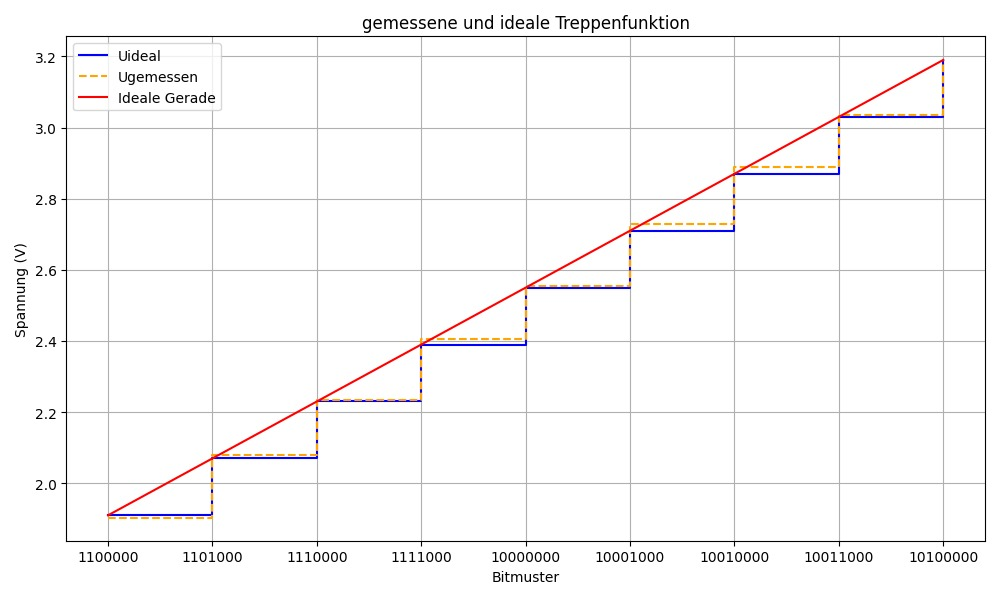
\includegraphics[width=1.0\textwidth]{../Quellen/Labor1/Versuch1/Treppenfunktion1.png}
    \caption{Treppenfunktionen ideale und gemessene Spannung mit Ideal-Gerade}
\end{figure}



\subsubsection*{Messung der Konversionsrate}
Der letzte Teilversuch des ersten Experiments bestand darin, für eine mittlere Eingangsspannung die tatsächliche Zykluszeit und Frequenz für die Clock, sowie für die Konversion des ADCs zu messen. Des Weiteren sollte die Anzahl der benötigten Clock-Zyklen für eine Konversion in Erfahrung gebracht werden.\\
Für diese Messungen wurde das Oszilloskop benötigt und mit Bananenkabeln mit dem Steckbrett verbunden. Die Konversionszeit wurde bestimmt, indem durch den Pin 3 (den Write) und Pin 5 (dem Interrupt) der Start und das Ende der Koversion gemessen wurde. Der Beginn einer Konversion zeigt sich durch den Wechsel von Low auf High am Pin 3. Das Ende der Konversion zeigt der Interrupt bei Pin 5 durch einen Wechsel auf Low. Die Zykluszeit wird an der Clock, an Pin 4, gemessen. All die Messungen konnten am Oszilloskop und durch Rechnungen entwertet werden (siehe Figure 5 und 6).


\begin{figure}[H]
    \centering
    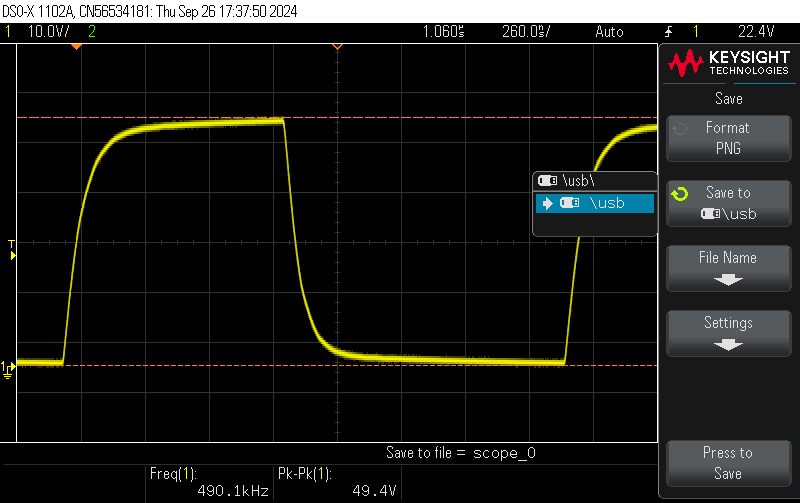
\includegraphics[width=0.9\textwidth]{../Quellen/Labor1/Versuch1/scope_0.png}
    \caption{Zykluszeit}
\end{figure}


\begin{figure}[H]
    \centering
    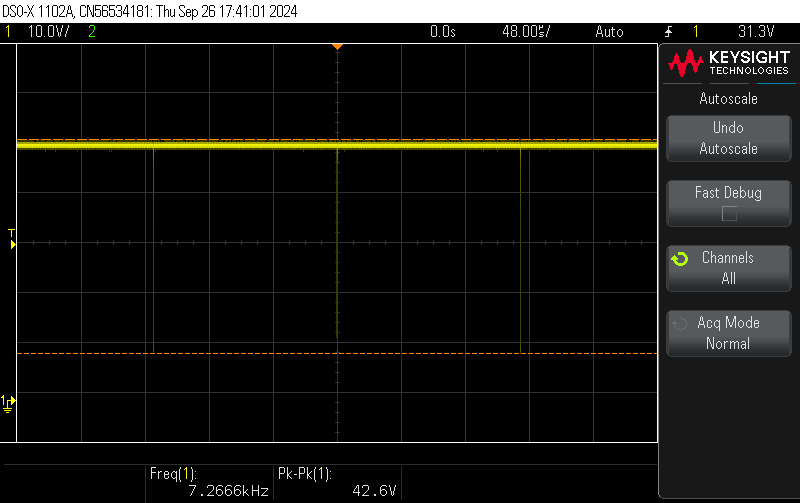
\includegraphics[width=0.9\textwidth]{../Quellen/Labor1/Versuch1/scope_1.png}
    \caption{Koversionszeit}
\end{figure}

Die gemessenen und berechneten Werte sind in folgender Tabelle (Table 3) aufgeführt:
\setlength{\tabcolsep}{12pt}
\begin{table}[H]
    \centering
    \begin{tabular}{|c|c|c|}
	\hline
        	 & Messung & Datenblatt\\
	\hline
	Clock-Zykluszeit & 2.04 µs & 1.56 µs\\
	Clock-Frequenz & 490 kHz & 640 kHz\\
	Konversionszeit & 137 µs & 103 - 114 µs\\
	Konversionsfrequenz & 7.27 kHz & 8.77 - 9.71 µs\\
	Anzahl Clock-Zyklen & 67 & 66 - 73\\
	\hline
    \end{tabular}
    \caption{Messergebnisse im Vergleich mit dem Datenblatt}
\end{table}
\noindent Zuletzt wurden die gemessenen Daten, mit den Werten des Datenblatts abgeglichen. Die Abweichungen zwischen den gemessenen Werten, Clock-Zykluszeit und Konversionszeit, und dem Datenblatt, lassen sich durch die Abweichung der Clock-Frequenz erklären. Es gab die Möglichkeit ab einer bestimmten Frequenz den 10 k$\Omega$-Widerstand mit einem 5,1 k$\Omega$-Widerstand zu ersetzen. Da die gemessene Frequenz den besagten Wert aber stark übersteigt, müssen die Abweichungen so hingenommen werden. Des Weiteren sind die Abweichungen nicht hoch und beide Abweichungen sind höher als der Wert aus dem Datenblatt. Außerdem liegt die Anzahl der Clock-Zyklen im vorgesehenen Bereich und die Konversionsfrequenz ist nur geringfügig kleiner als die vorgesehene.
\newpage




\section{Versuch 2: DAC}

\subsection{Zielsetzung}
In diesem Versuch sollte die Funktionsweise eines Digital/Analog-Wandlers (DAC) untersucht werden. Der Fokus lag auf der Bestimmung wichtiger Parameter wie Monotonie, Linearität und Einschwingzeit, um die Leistungsfähigkeit des DAC zu evaluieren.
\begin{itemize}
    \item \textbf{Monotonie} beschreibt die Eigenschaft eines DAC, bei einer stetigen Erhöhung des digitalen Eingangswerts immer auch eine stetig ansteigende analoge Ausgangsspannung zu erzeugen. Es darf keine abfallenden Werte geben.

    \item \textbf{Linearität} bewertet, wie gut der DAC die digitalen Eingangswerte in proportionale analoge Ausgangswerte umwandelt. Eine ideale Linearität bedeutet, dass jeder Schritt in der digitalen Eingabe zu einer exakt gleich großen Veränderung der Ausgangsspannung führt. Abweichungen von dieser Idealgeraden müssen erfasst und analysiert werden, um die Genauigkeit des Wandlers zu bewerten.

    \item \textbf{Einschwingzeit} beschreibt die Zeit, die der DAC benötigt, um nach einer Änderung des digitalen Eingangswerts eine stabile Ausgangsspannung zu erreichen. Dieser Parameter ist besonders wichtig für Anwendungen, in denen schnelle und präzise Spannungsänderungen erforderlich sind.
\end{itemize}

\noindent Der Versuch hatte das Ziel, die Messungen dieser Parameter durchzuführen, um zu prüfen, wie gut der DAC den Anforderungen an präzise analoge Signalumwandlung gerecht wird. Die ermittelten Werte sollten mit den theoretischen Erwartungen aus dem Datenblatt des Herstellers verglichen und eventuelle Abweichungen dokumentiert werden.

\subsection{Bauteile und Messgeräte}
Verwendete Geräte und Zubehör:
\begin{itemize}
\item Netzgerät (NEP-8323)
\item Fluke 87 V True RMS Multimeter
\item Keysight Oszilloskop (DSOX1102A)
\item Bananenkabel (mehrere: rot, blau, schwarz)
\item Sicherheits-Klemmprüfspitze (2 Stück)
\item Oszilloskop BNC Tastkopf mit Masseklemme
\item Steckkabel (mehrere: im Idealfall verschiedene Farben)
\item Steckbrett\\
\end{itemize}

\noindent Verwendete Bauteile:
\begin{itemize}
\item Digital/Analog-Wandler (DAC ZN429E-8)
\item D-Flip-Flop (SN74LS74AN)
\newpage
\item Kondensatoren: 
	\begin{itemize}
	\item 10 µF "Tantalum"
	\item 0,1 µF
	\end{itemize}
\item Widerstände: 
	\begin{itemize}
	\item 1k$\Omega$
	\item 8 x 1 k$\Omega$ Widerstandsnetzwerk
	\end{itemize}
\end{itemize}

\subsection{Messkonzept}
Das Messkonzept für die Untersuchung des DAC's basierte auf der Überprüfung der Monotonie, Linearität und Einschwingzeit. Um diese Parameter zu ermitteln, wurde eine Schaltung nach einer eigens entworfenen Schaltskizze aufgebaut, die den grundlegenden Aufbau des Versuchs zeigt und während des gesamten Experiments unverändert blieb. Das Ziel war es, die Eigenschaften des DAC systematisch zu untersuchen, indem verschiedene digitale Werte an den Eingang des DACs angelegt und die entsprechenden analogen Ausgangswerte gemessen wurden.

\subsubsection {Schaltung und Schaltskizze}

Die Schaltung bestand aus dem DAC und einem D-Flip-Flop zur Synchronisierung der digitalen Eingangssignale. Die Schaltskizze (siehe Anhang) zeigt den Teil des Aufbaus, der während des gesamten Versuchs unverändert blieb, einschließlich der Verbindungen für die Versorgungsspannung und die Masseleitungen.\\
\noindent Die digitalen Werte, die an den DAC gesendet wurden, mussten über Steckkabel in die entsprechenden Pins eingefügt werden. Dies ermöglichte eine schrittweise Änderung der digitalen Eingangswerte.

\begin{figure}[H]
    \centering
    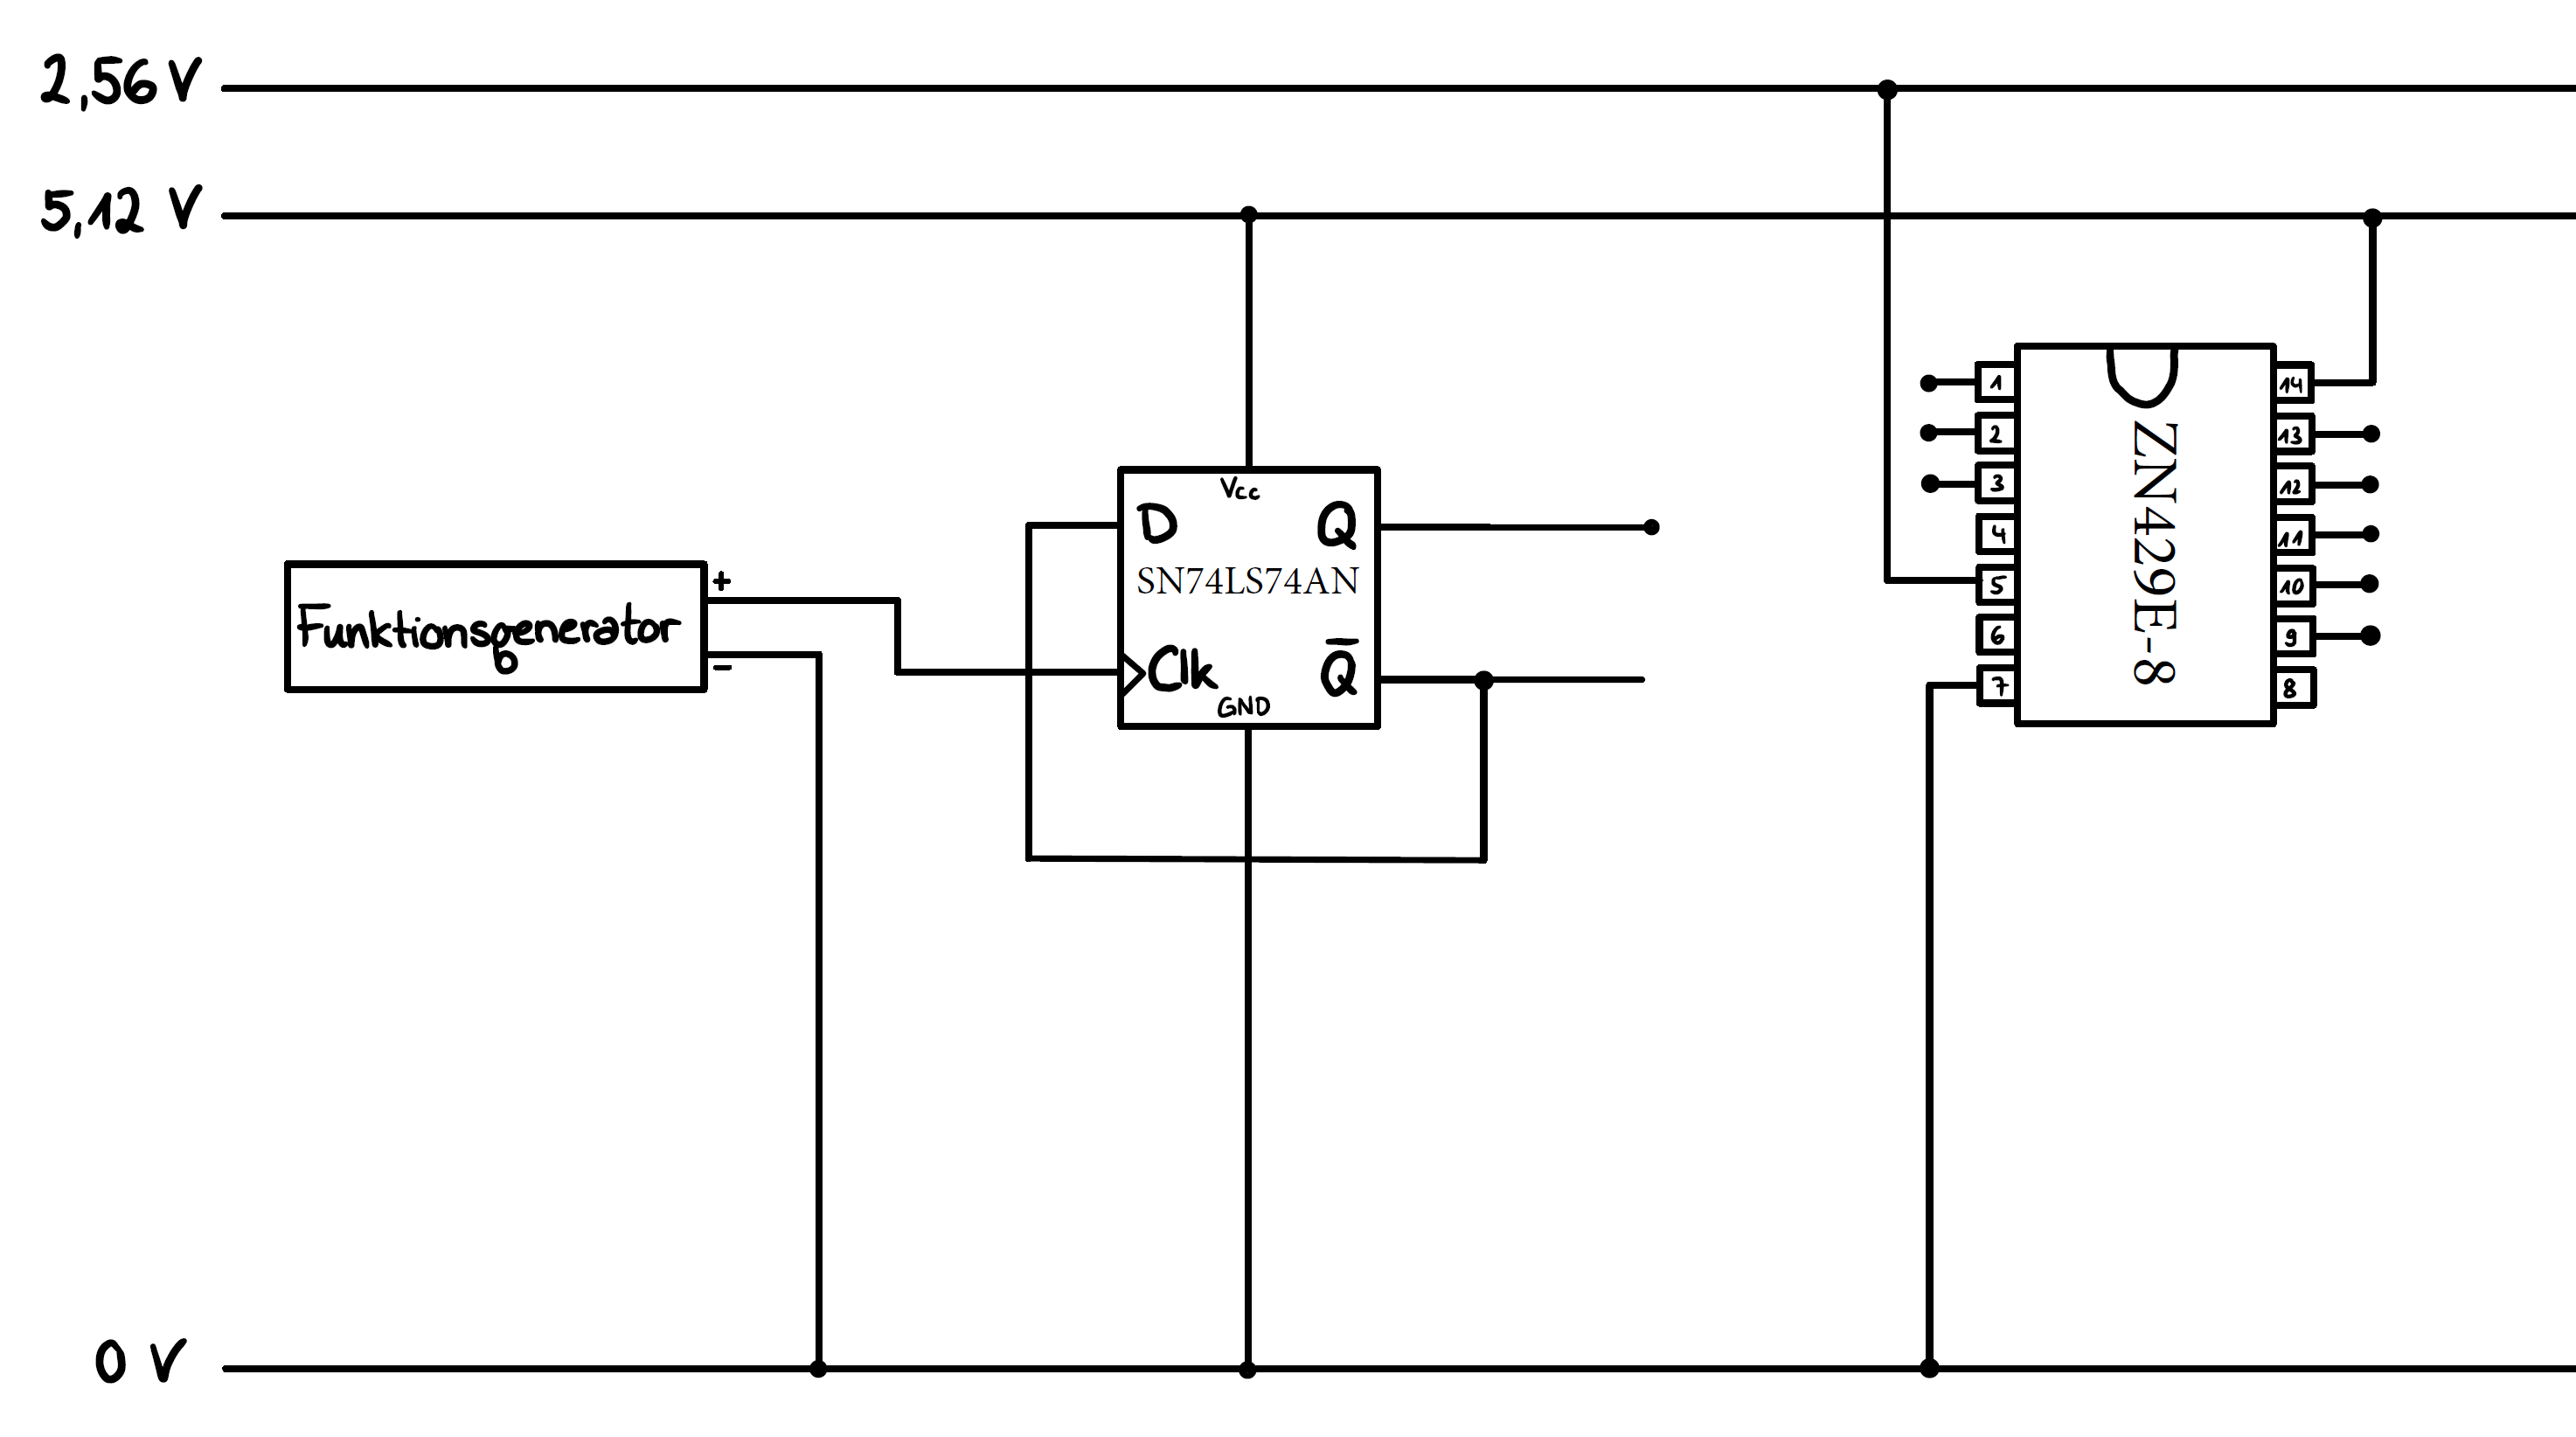
\includegraphics[width=1\textwidth]{../Quellen/Labor1/Versuch2/Schaltskizze.png}
    \caption{Schaltskizze des Messaufbaus}
\end{figure}

\subsubsection {Monotonie- und Linearitäts-Messung}

Für die Messung der Monotonie und Linearität des DAC wurde der digitale Eingabewert systematisch verändert, indem nacheinander die Bitmuster an den Eingang des DAC gelegt wurden. Bei jedem Schritt wurde die analoge Ausgangsspannung gemessen, um beide Eigenschaften zu prüfen. Die Monotonie wurde überprüft, indem untersucht wurde, ob die Ausgangsspannung bei jeder Erhöhung des digitalen Werts ohne Abfall kontinuierlich steigt. Gleichzeitig wurde die Linearität bewertet, indem die gemessenen Ausgangsspannungen mit den theoretisch erwarteten Werten verglichen wurden, um Abweichungen zur Idealgeraden zu berechnen.

\noindent Messung der Signale am Oszilloskop: Das Oszilloskop wurde verwendet, um das Ausgangssignal des DAC zu überwachen. Es wurde direkt mit dem Bitsprung des DAC-Ausgangs getriggert, um sicherzustellen, dass jede Änderung im digitalen Eingabewert präzise erfasst wurde.

\noindent Monotonieprüfung: Bei dieser Messung wurde untersucht, ob das Bauteil durchgängig monoton arbeitet, d. h. bei jedem Bitwechsel nur steigende oder gleichbleibende Ausgangsspannungen erzeugt, ohne dass die Spannung zwischenzeitlich abfällt.

Die Linearität des DAC wurde ebenfalls während der gleichen Messung bestimmt. Die Referenzspannung wurde mit 2,56 V gewählt.

\noindent Messung mit dem Multimeter: Die gemessenen Ausgangsspannungen für verschiedene digitale Eingabewerte wurden mit einem Fluke DMM aufgenommen und in einer Tabelle dokumentiert, um sowohl Monotonie als auch Linearität bewerten zu können.

\begin{figure}[H]
    \centering
    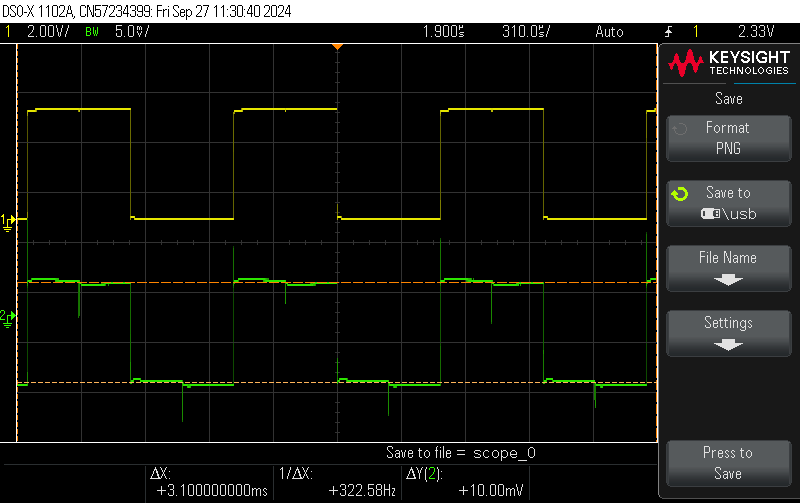
\includegraphics[width=1\textwidth]{../Quellen/Labor1/Versuch2/scope_0.png}
    \caption{Monotonie- und Linearitäts-Messung}
\end{figure}

\begin{figure}[H]
    \centering
    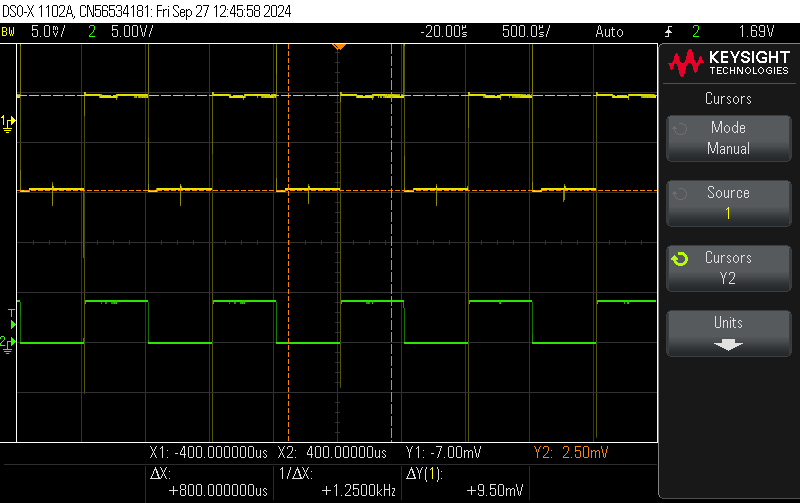
\includegraphics[width=1\textwidth]{../Quellen/Labor1/Versuch2/scope_2.png}
    \caption{Monotonie- und Linearitäts-Messung}
\end{figure}

\subsubsection {Einschwingzeit-Messung}

Die Einschwingzeit des DAC beschreibt die Zeit, die der Wandler benötigt, um nach einem digitalen Sprung (z.B. von einem niedrigen auf einen hohen Wert) eine stabile Ausgangsspannung zu erreichen.\\
\noindent Messung der Einschwingzeit: Für diese Messung wurde ein Bitwechsel (Sprung im digitalen Eingabewert) erzeugt und die Reaktion des DAC-Ausgangs wurde mit dem Oszilloskop aufgezeichnet. Die Einschwingzeit wurde gemessen, ab dem Zeitpunkt, bei dem die letzte Konversion abgeschlossen wurde, bis die Ausgangsspannung stabil war.

\begin{figure}[H]
    \centering
    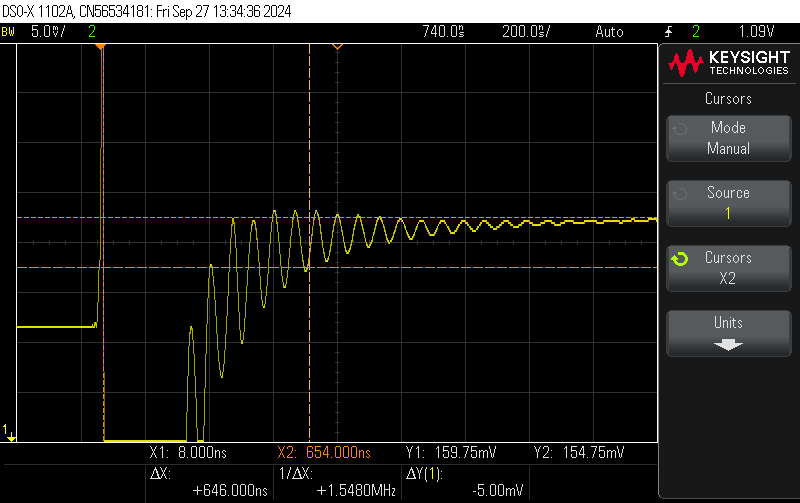
\includegraphics[width=1\textwidth]{../Quellen/Labor1/Versuch2/scope_3.png}
    \caption{Einschwingzeit-Messung}
\end{figure}

\begin{figure}[H]
    \centering
    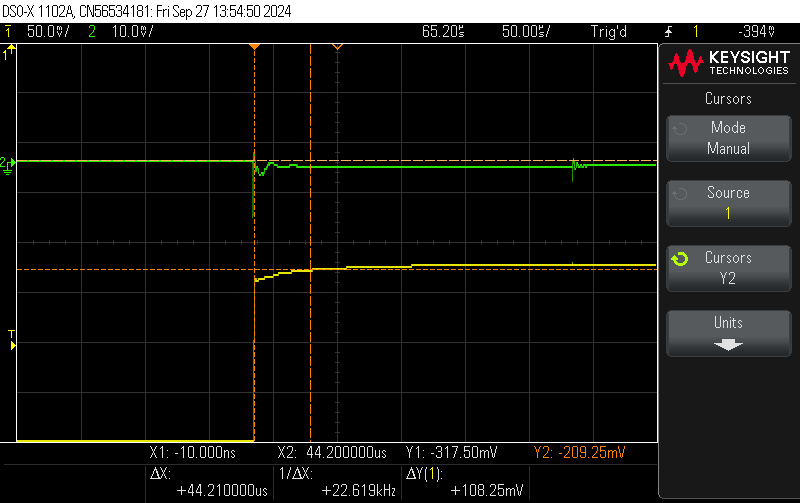
\includegraphics[width=1\textwidth]{../Quellen/Labor1/Versuch2/scope_5.png}
    \caption{Einschwingzeit-Messung}
\end{figure}

\subsection{Messergebnisse}

\begin{table}[H]
    \centering
    \begin{tabular}{|c|c|c|}
        \hline
        Bitsprung & \( \Delta U_{DAC} \) & Monoton? \\
        \hline
        00000001 & 10 mV & Ja \\
        00000010 & 10,25 mV & Ja \\
        00000100 & 10,25 mV & Ja \\
        00001000 & 10 mV & Ja \\
        00010000 & 10 mV & Ja \\
        00100000 & 10 mV & Ja \\
        01000000 & Fehler am Steckbrett & - \\
        10000000 & Fehler am Steckbrett & - \\
        00000000 & Fehler am Steckbrett & - \\
        \hline
    \end{tabular}
    \caption{Messergebnisse für Monotonie- und Linearitätsmessung}
\end{table}


\subsection{Diskussion}
Diskutiere die Messergebnisse. Was sind die wichtigsten Erkenntnisse? Was lief gut, was könnte verbessert werden?

\section{Fazit}
Ziehe ein Fazit über die Laborversuche. Was wurde gelernt? Welche Herausforderungen gab es?

\end{document}
